Clase: 11/10/2022

\begin{teorema}[De convergencia analítica]
    Sea $A$ un conjunto abierto de $\mathbb{C}$ y sea $(f_n)$ una sucesión de funciones analíticas definidas sobre $A$. Si $f_n \to_{unif} f$  sobre cada disco cerrado contenido en $A$, entonces $f$ es analítica. Además, $f_n'\to f'$ puntualmente sobre $A$ y uniformemente sobre cada disco cerrado en $A$. 
    \begin{dem}
        Tenemos 
        \begin{enumerate}
            \item Sea $z_0\in A$ y sea $B=\{z:\underbrace{|z-z_0|}_{\in A}\leq r\}=D_r[z_0]\subseteq A$
            \item Nótese que $D_r[z_0]$ es simplemente conexo. 
            \item Como $f_n\to_{unif}f$ sobre cada $D_r[z_0]\implies f_n\to_{unif}f$ sobre $D_r(z_0)$.
            \item  Como $f_n$ es analítica, $\forall n\in \mathbb{Z}^+\implies f_n$ es continua. Entonces, $f$ es continua en el disco abierto $D_r(z_0)$. 
        \end{enumerate}
        $\implies$ como $f_n$ es analítica sobre el simplemente conexo $D_r(z_0)$, por el teorema de Cauchy $\int_\gamma f_n=0$, para cualquier curva cerrada $\gamma$ en $D_r(z_0)$. Entonces por la propiedad anterior, $\int_\gamma f=0$, y por Morera, $f$ es analítica sobre $D_r(z_0)$.
    \end{dem}

    \begin{dem}
        Sea 
        \begin{enumerate}
            \item Sea $z_0\in A$ y sea $B=\{z:\underbrace{|z-z_0|}_{\in A}\leq r\}=D_r[z_0]\subseteq A$. 
            \item Sea $\gamma$ centrado en $z_0$ y con radio $\rho >r$ y contenido en $A$. 
            \begin{figure}[H]
                \centering
                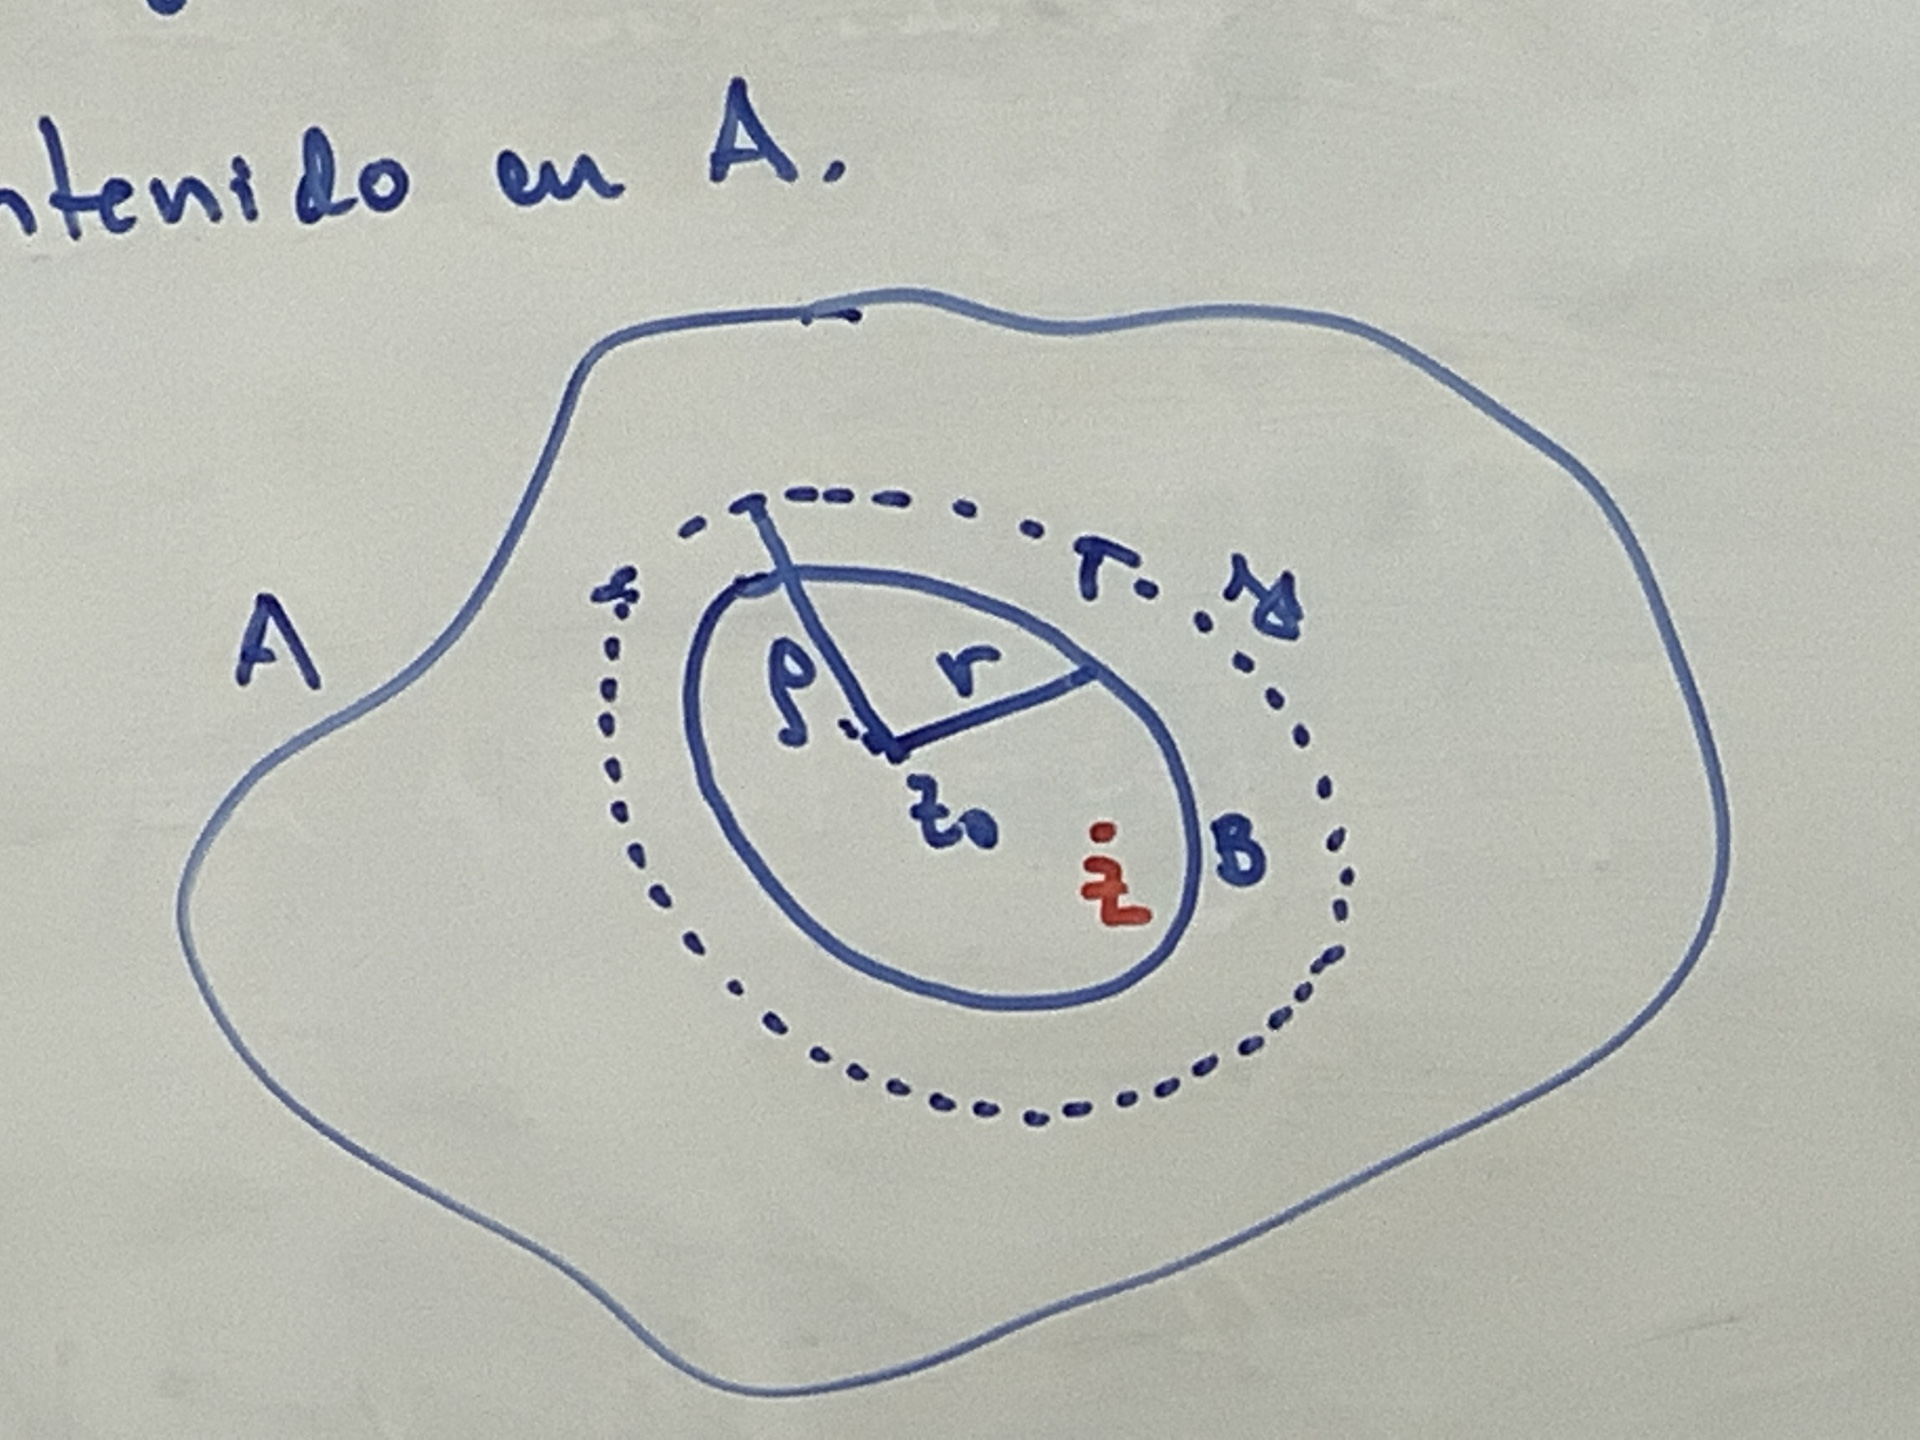
\includegraphics[scale=0.1]{imagenes/19.1.jpeg}
            \end{figure}
            $\forall z\in B$, se tiene: 
            \begin{align*}
                f_n'(z) &= \frac{1}{2\pi i}\int_\gamma \frac{f_n(\psi)}{(\psi - z)^2}d\psi 
            \end{align*}
            y 
            \begin{align*}
                f'(z) &= \frac{1}{2\pi i}\int_\gamma \frac{f(\psi)}{(\psi - z)^2}d\psi 
            \end{align*}
            \item Como $f_n\to_{unif} f$ sobre discos cerrados en $A\implies f_n\to_{unif}f$ es $\{z:|z-z_0|\leq \rho\}\subset A\implies$ Dado $\varepsilon>0\exists N\in \mathbb{Z}^+\ni$ si $n\geq N\implies |f_n(\psi)-f(\psi)|<\varepsilon,\forall \psi \in \gamma$
            \item Entonces, 
            
            \begin{align*}
                |f_n'(z)-f'(z)| &=\left|\frac{1}{2\pi i}\frac{f_n(\psi)-f(\psi)}{(\psi - z)^2}d\psi\right|\\
                &\leq \frac{1}{2\pi}2\pi \rho
            \end{align*}
            \begin{cajita}
                Se tiene: 
                \begin{align*}
                    \left|\frac{f_n(\psi)-f(\psi)}{(\psi - z)^2}\right| &\leq \frac{\varepsilon}{|\psi -z|^2}\left[\frac{\varepsilon}{(p-r)^2}\right]\\
                    &= \frac{\varepsilon \rho}{(\rho-r)^2}
                \end{align*}
                con $|\psi -z|>\rho -r\implies \frac{1}{|\psi - z|}<\frac{1}{\rho-r}$
            \end{cajita}
        \end{enumerate}
    \end{dem}
\end{teorema}

\begin{ejemplo}
    Muestre que la función $\zeta$ de Riemann definida 
    $$\zeta(z)=\sum_{n=1}^{\infty}n^{-z}$$
    es analítica sobre $A=\{z:\operatorname{Re} z>1\}$
    \begin{cajita}
        Hipótesis de Riemann(1859): Todos los ceros no triviales de $\zeta(z)$ tienen parte real igual a $1/2$.
    \end{cajita}
    \begin{figure}[H]
        \centering
        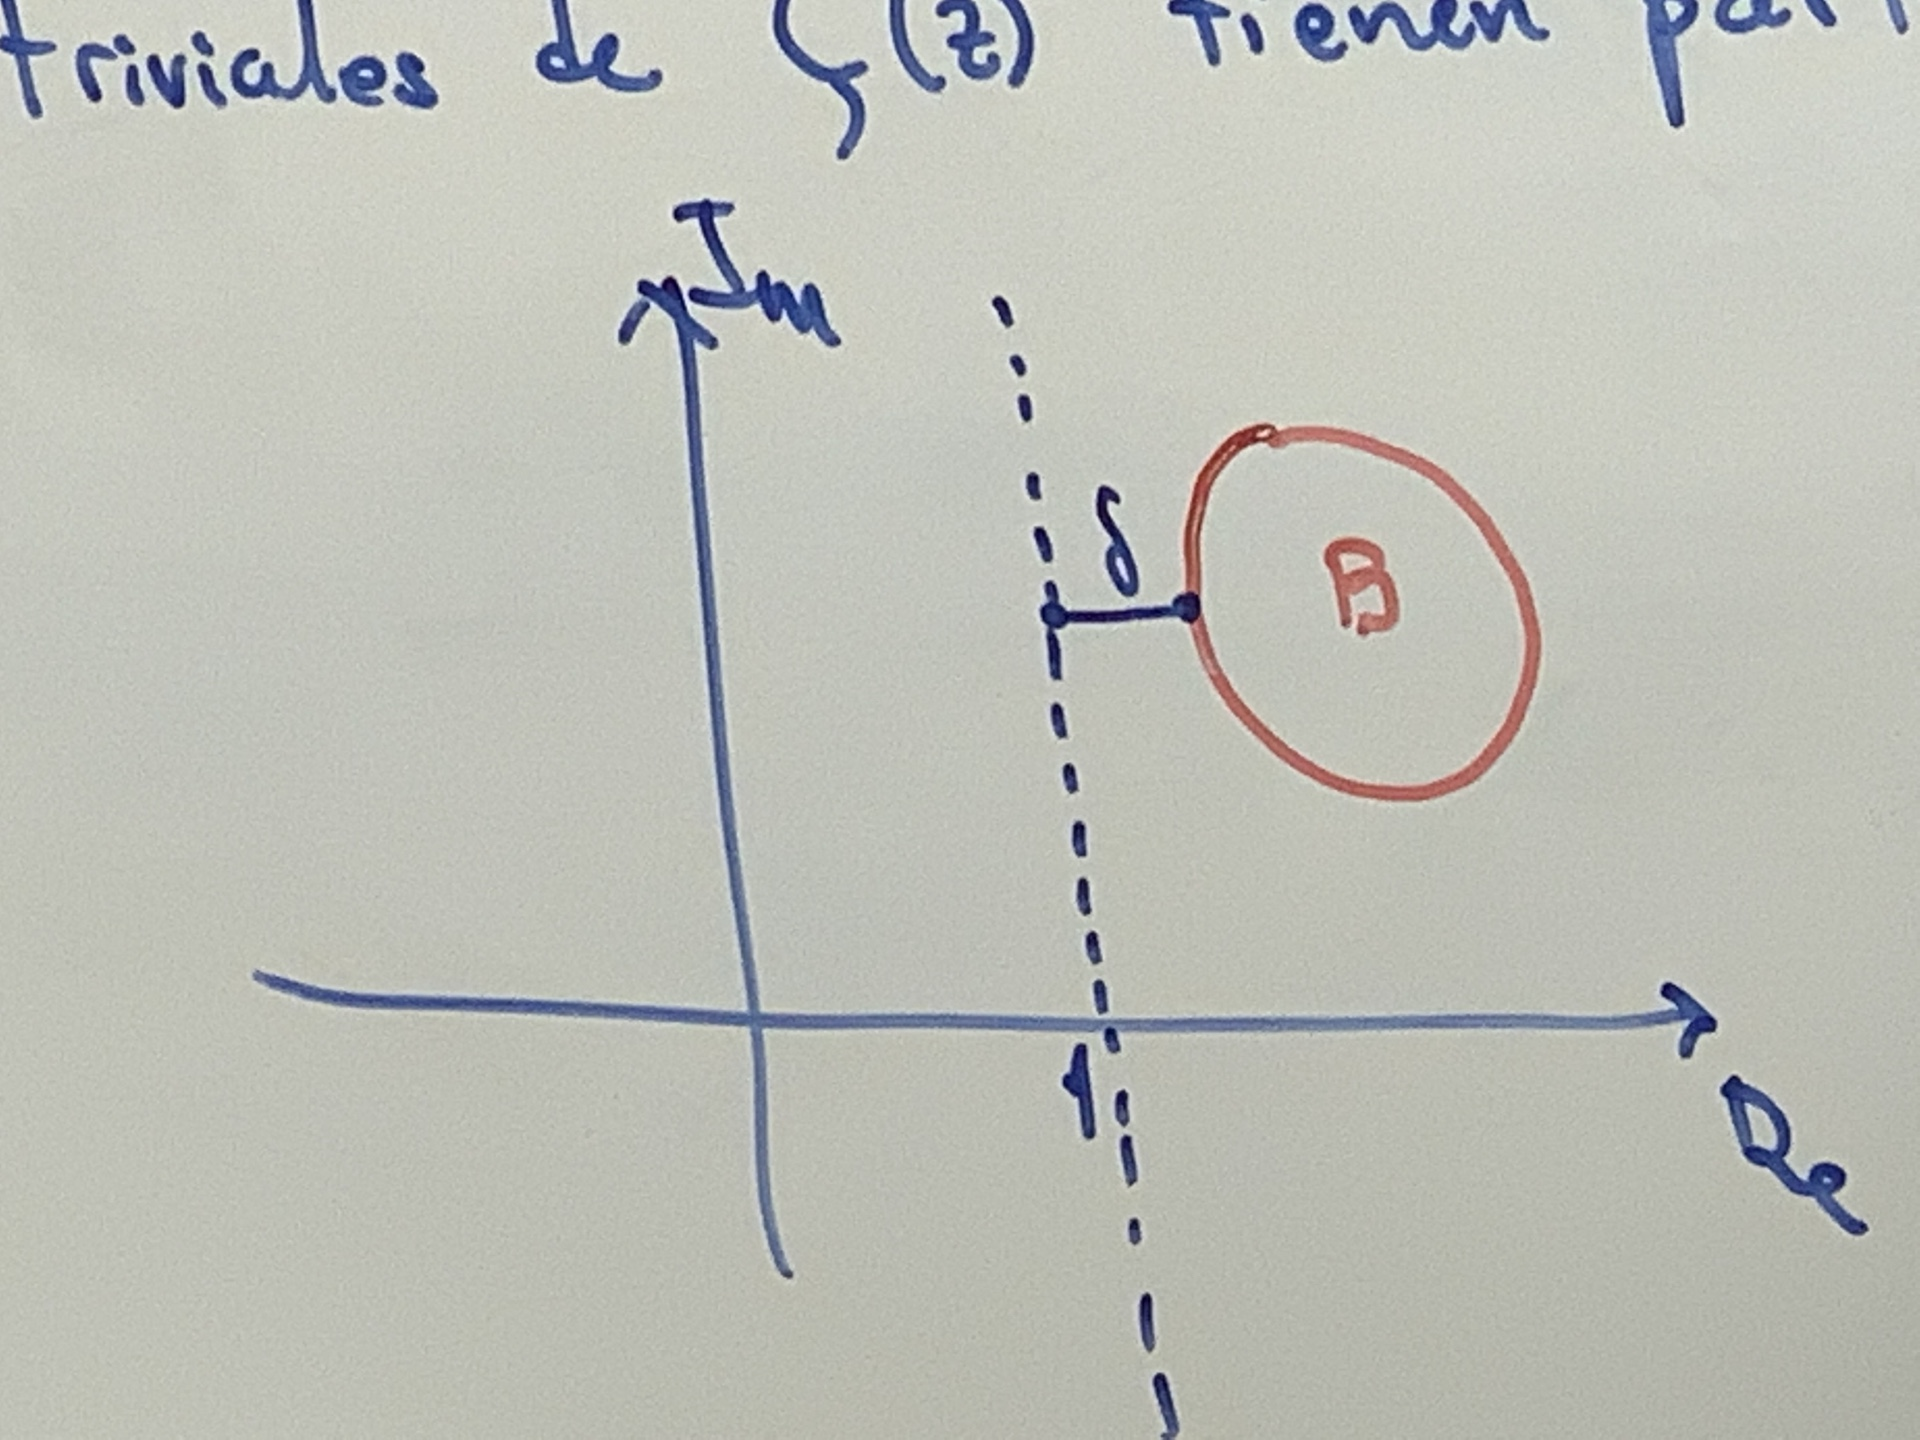
\includegraphics[scale=0.1]{imagenes/19.2.jpeg}
    \end{figure}  con distancia $\delta$
    \begin{sol}
        Sea $B$ un disco cerrado contenido en $A$ y con distancia $\delta$ de la vertical $\operatorname{Re}z=1$. A probar: $\sum_{n=1}^{\infty} n^{-z}$ converge uniformemente sobre $B$. 
        Nótese que, si $z=x+iy\in B$, entonces
        \begin{align*}
            |n^{-z}| &= |e^{-z\log n}|\\
                    &= |e^{-(x+iy)\log n}|\\
                    &=| e^{-x\log n}|= n^{-x}, x\geq 1+\delta
        \end{align*}
        Entonces, si $z\in B\implies |n^{-z}|\leq n^{-(1+\delta)}=M_n$. 
        Además, $\sum_{n=1}^{\infty}\frac{1}{n^{1+\delta}}$ converge por $p$-series $\implies$ por $M$-test se tiene $\zeta(z)$ converge uniformemente sobre cada disco cerrado $B\subseteq A\implies \zeta(z)$ es analítica sobre $A$. 
    \end{sol}
\end{ejemplo}

\section{Producto cartesiano generalizado}

Sea $X_\alpha$ un conjunto $\forall a\in A$. El producto cartesiano de los $X_\alpha$ es el conjunto 
$$\prod_{\alpha \in A}X_{\alpha}=\left\{ x:A\to \bigcup_{\alpha \in A}X_\alpha: x(\alpha)\in X_\alpha, \forall \alpha\in A\right\}$$

\begin{ejemplo}
    Sea $A=\{1,2\},X_1=\{a,e,i\},X_2=\{o,u\}$.
    \begin{enumerate}
        \item Primera función
        \begin{align*}
            X_1(1) &= a\\
            X_1(2) &= o
        \end{align*}
        \item Segunda función
        \begin{align*}
            X_2(1) &= a\\
            X_2(2) &= u
        \end{align*}
        \item Tercera función
        \begin{align*}
            X_3(1) &= e\\
            X_3(2) &= o
        \end{align*}
        \item Cuarta función
        \begin{align*}
            X_4(1) &= e\\
            X_4(2) &= u
        \end{align*}
        \item Quinta función
        \begin{align*}
            X_5(1) &= i\\
            X_5(2) &= o
        \end{align*}
        \item Sexta función
        \begin{align*}
            X_6(1) &= i\\
            X_6(2) &= u
        \end{align*}
    \end{enumerate}
\end{ejemplo}